\chapter{Methodology}
This section lays out the methodology behind the signal detection of ICESat-2 signal, the interpolation of the sparse signal points into depth and uncertainty grids, and how these grids are combined with GEBCO to produce an upscaled version.
\section{Test Cases}
To test the methodology, a series of test sites were selected, based on the suitability of the site (i.e. clear water), and the availablity of high-resolution in-situ bathymetry. Additionally, to test the kriging interpolation accuracy, a test site in Petten, The Netherlands was used.
\subsection{Petten, NL}
The Netherlands provides a dataset called Jarkus that contains surveyed measurements of the nearshore zone and the dunes along a set of fixed transects along the dutch coast. Additionaly, a recently-surveyed, high-resolution bathymetric grid of the coast off Petten, NL was provided by Van Oord. Using this data, the kriging interpolation method, and the Kalman update was tested to see if it can increase the accuracy of resampled GEBCO. 
\subsection{Florida Keys, FL, USA}
\subsection{Oahu, HI, USA}
\subsection{Maldives}

\section{Identification of bathymetric signal in ICESat-2 data} \label{sec:kdesignalfinding}
Most of the studies that try to find bathymetric points from ICEsat-2 use some variation of the DBSCAN algorithm to identify possible bathymetric signal. The algorithm has the advantages of being robust to noise \cite{} and computationally efficient. However, one disadvantage is that is is very sensitive to the choice of parameter values, and setting them programmatically so that they work on a global scale basis is difficult. \pdfcomment{does this statement need better support?}, and some previous studies employing the DBSCAN method used a manual correction after classification to remove clusters of noise incorrectly labeled as signal (e.g. \cite{Ma2020}). Also, methods based on DBSCAN label points as either likely signal or noise, but then require interpolation of the Z values to calculate a sea surface value from the identified signal photons. Therefore, a novel \pdfcomment{nope} method is proposed to find areas of likely signal and extract the seafloor elevation in a single step, based on a kernel density estimation algorithm that is applied along a rolling window along the transect.

The proposed steps of this method are:
\subsection{Filter to subsurface photons}

The raw photon cloud from the ATL03 data product contains photons returns from land, clouds, the sea surface, and noise photons. Before applying an algorithm to extract bathymetric signal from noise, first areas of the photon cloud that could not contain bathymetric signal must be removed. A filtering algorithm was developed to cull points in the following order:

\begin{enumerate}
    \item For each point, extract the elevation from the GEBCO dataset. Any points have a GEBCO elevation value of greater than +6m or less than -50m are removed. It is assumed that any points with a GEBCO elevation greater than 6 meters are assumed to be land, and any points where the GEBCO elevation is less than -40m are assumed to be outside the limit of ICESat-2's maximum range for bathymetric sensing (The deepest bathymetric depth known to be detectable by ICESat-2 is 38m. \parencite{Parrish2019})
    
    \item Any points with an elevation greater than 5m above the geoid are assumed to be high noise or land, and are removed from the point dataset.

    \item Calculate the sea surface for each point along the transect. This can be done using the rolling median of the remaining points with window width of 200 points that are marked as high confidence ocean signal \parencite{Ranndal2021}. Then subtract the Z elevation to get the depth below the ocean surface.  Cull any points deeper than 40m. 
    % This provides the vertical filtering. 
    \item Cull any points within a buffer distance of the sea surface. This removes the strong signal associated with the sea surface.
\end{enumerate}

An example input to the process above is shown in \ref{fig:filtering_results}. The points remaining after the filtering are shown in 

\begin{figure}[h!]
    \centering
    \includegraphics[width=\textwidth]{figures/filtered_vs_unfiltered.jpg}
    \caption{All photons geolocations along a single transect}
    \label{fig:filtering_results}
\end{figure}

\begin{figure}[h!]
    \centering
    \includegraphics[width=\textwidth]{figures/photons_after_filtering.jpg}
    \caption{Points remaining after filtering}
    \label{fig:filtered_pts_only}
\end{figure}

The filtering steps reduce the dataset to just photon locations that are in the subsurface zone. To determine if there is bathymetric signal present, further processing is required. There have been several methods for separating bathymetric signal photons from noise, which are explained in section \ref{subsec:denoising}. For this project\pdfcomment{reword?}, a new method is proposed based on a Gaussian Kernel Density Estimation (KDE) function. A function is created that returns the maximum kernel density, and the Z location at which it occurs. Figure \ref{fig:kdefunc} shows the KDE function as applied to two different windows, and the resulting kernel density plots. The KDE function is highly influenced by the \emph{Bandwidth} parameter. For this implementation, the Scott method \parencite{Scott2015} is used to estimate the required bandwidth based on the data. 

This function is applied on a rolling basis to a window of 200 points. This function returns a value for every single point along the transect, including in areas that do not have any noticeable signal. The kernel density value gives an indication of the strength of the peak. To reject the locations where the signal is weak, any points with a KDE value of less than the median value $$ kde_{50} $$ \pdfcomment{maybe just less than median? that decreases RMS error at the florida site} are assigned an NaN value and are dropped from the analysis.

\begin{figure}[htbp]
    \centering
    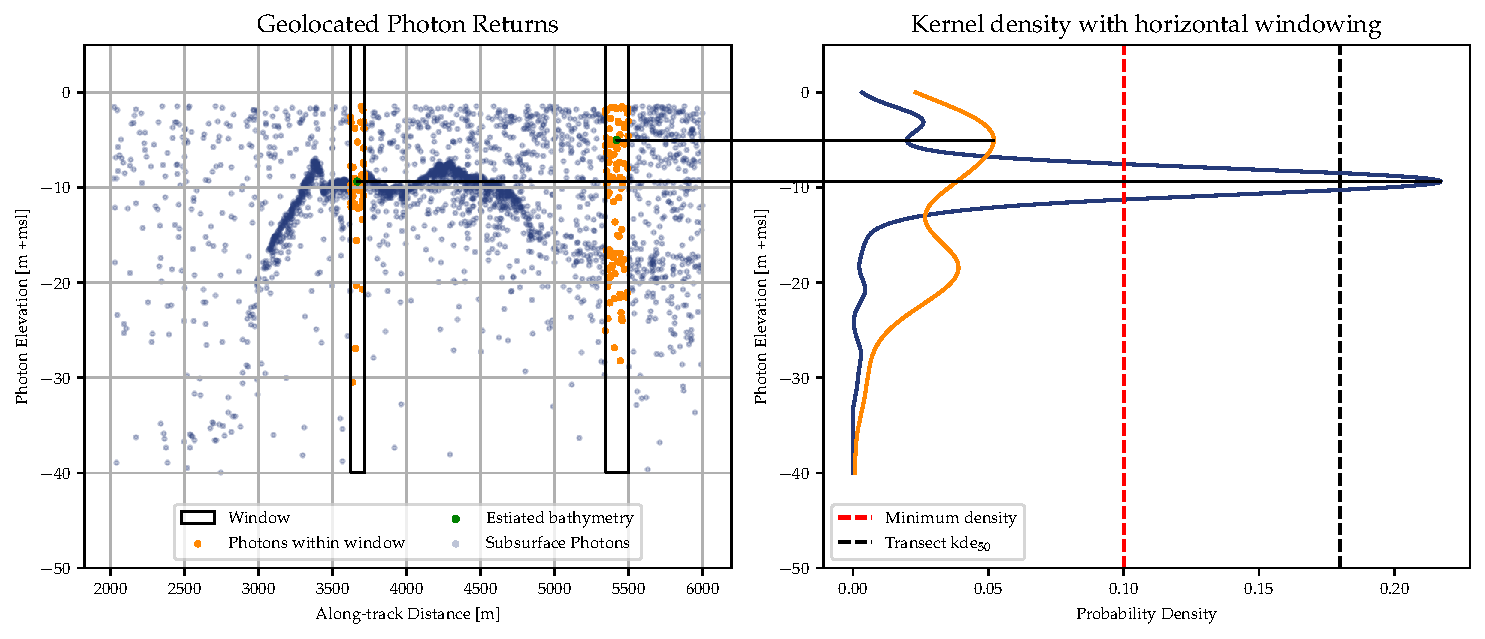
\includegraphics[width=\textwidth]{figures/2d_kde_plot.png}
    \caption{KDE function as applied to 2 different windows}
    \label{fig:kdefunc}
\end{figure}

The input parameters to the signal finding function are:

\begin{enumerate}
    \item The size of the window in \emph{number of points}
    \item the cutoff value for the Kernel Density required for point to be considered signal
\end{enumerate}

\section{Interpolation of Bathymetric Point Data to Raster Data}

After the bathymetric signal points are identified per the method in \ref{}, the resulting bathymetry points are densely spaced along satellite tracklines, but are absent between them. To convert these densely-spaced vector point locations to a raster of elevation data, and a raster of uncertainty data, geostatistical measures are used.

\subsection{Subsampling of Bathymetric points using Poisson Disk Sampling} \label{subsec:poissonsubsampling}
The bathymetric points are extremely densely spaced, and kriging algorithms are computationally expensive. To reduce the number of points fed into the algorithm, a subsample of the points is taken using the poisson disk sampling technique. 

\subsection{Kriging interpolation}
Using the subsample of the points from the poisson disk sampling, they are converted to a bathymetry raster using Universal Kriging. This geostatistical technique results in both a raster of the estimated depth as well as the estimated uncertainty. 


\section{Bayesian Data Assimilation using Kalman Filtering}
\subsection{Kalman Filter Background}
The Kalman Filter is a mathematical technique to predict the state of systems based on uncertain measurements. It consist of a loop of two steps, an \emph{Time update} step which updates the position based on a measurement and a known measurement uncertainty, and a \emph{measurement update} step which predicts the state based on the dynamic equations of the system. The kalman filter equations, for a state $x_k$ and a vector of measurements of the state $z_k$:

Time Update:

\begin{equation}
    \hat{x}_{\bar{k}} = A\hat{x}_{k-1} + B\hat{u_{k-1}}
\end{equation}

\begin{equation}
    P_{\bar{k}} = A P_{k-1} A^T + Q
\end{equation}

Measurement Update:
\begin{equation}
    K = P_{\bar{k}} H^T(H P_{\bar{k}} H^T + R) ^{-1}
\end{equation}

\begin{equation}
    \hat{x}_k = \hat{x}_{\bar{k}} + K(\hat{z}_k - H \hat{x}_{\bar{k}})
\end{equation}

\begin{equation}
    P_k = (I - KH)P_{\bar{k}}
\end{equation}


\subsection{Kalman Measurement Update Implementation}
The coastal zone is a highly dynamic system. However, for the purposes of this project is is assumed that the temporal variations over the time scale being studied are within the margin of error of the measurements, so the bathymetry of the nearshore zone is assumed to be a static system and the time update step can be ignored. It is also assumed all measurements are measurements of the same underlying physical depth, and that differences between measurements are due to normally distributed measurement error, with magnitude of the error varying depending on the method. To combine multiple measurements, the \emph{measurement update} step is applied recursively for each available measurement, producing a bayesian estimate of the bathymetry.  

